\newcommand{\DoNotLoadEpstopdf}{}
\documentclass[11pt,a4paper,landscape]{ltjsarticle}
\usepackage[margin=14mm,footskip=7mm]{geometry}
\usepackage{luatexja-fontspec}
\setmainfont{arial.ttf}[Path=C:/Windows/Fonts/,BoldFont=arialbd.ttf]
\setmainjfont{YuGothM.ttc}[Path=C:/Windows/Fonts/,FontIndex=0,BoldFont=YuGothB.ttc,BoldFeatures={FontIndex=0}]
\setsansjfont{YuGothM.ttc}[Path=C:/Windows/Fonts/,FontIndex=0,BoldFont=YuGothB.ttc,BoldFeatures={FontIndex=0}]
\usepackage{graphicx,booktabs,xcolor}
\definecolor{ink}{HTML}{263D50}
\setlength{\parindent}{0pt}
\setlength{\parskip}{5pt}
\newcommand{\heading}[2]{{\LARGE\bfseries\color{ink}#1}\par{\small #2}\par\vspace{2mm}}
\begin{document}
\heading{G70のCIM初期集団は、どこで改善が止まるのか}{交叉直後・局所探索後・集団への採用を、実際に生まれた子で確認した}
\begin{center}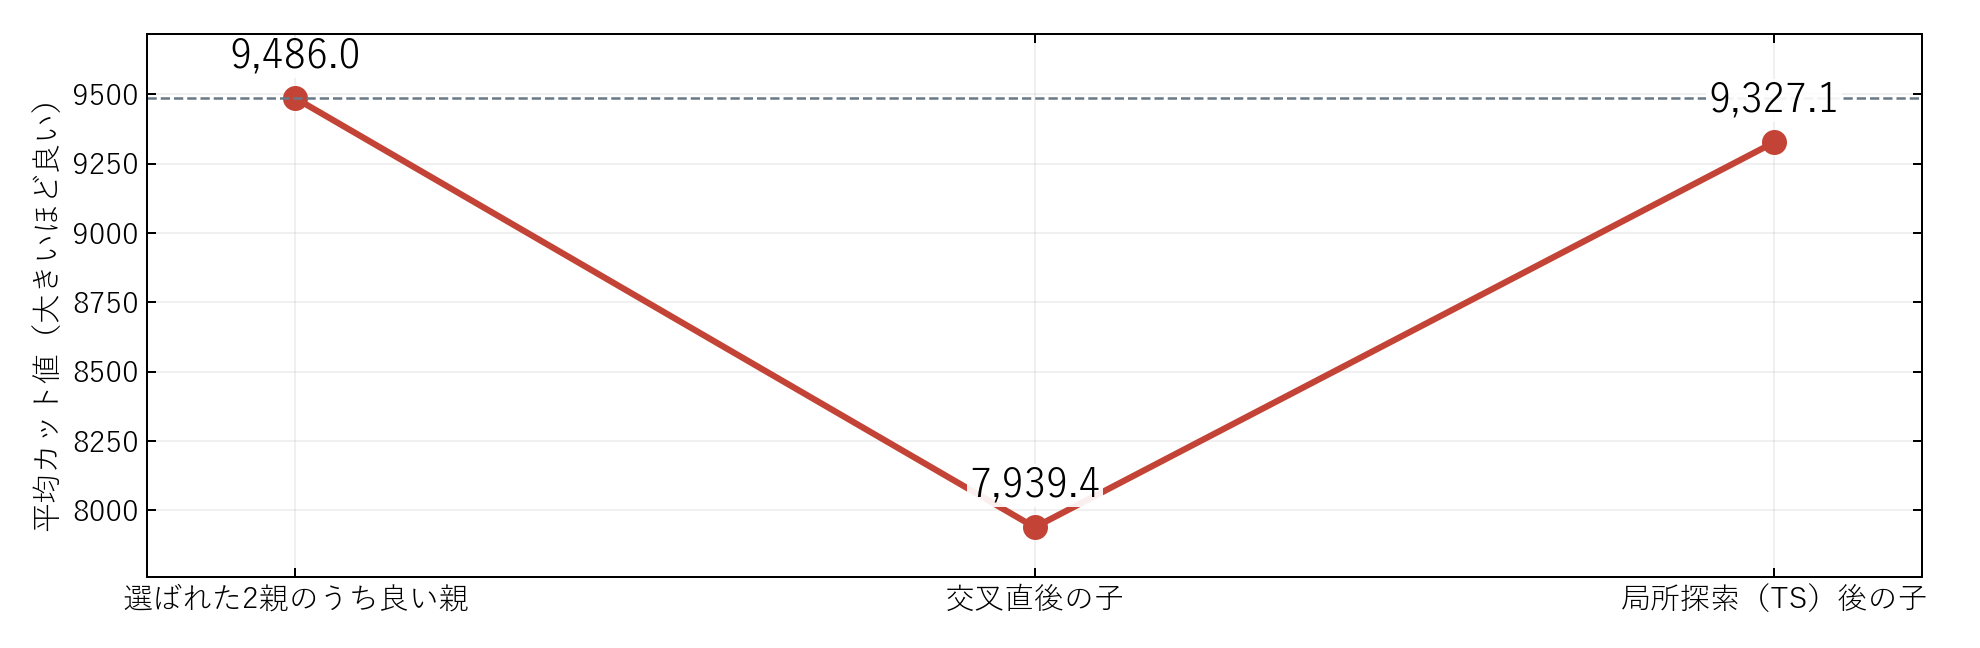
\includegraphics[width=.86\linewidth,height=74mm,keepaspectratio]{g70_stages.png}\end{center}
\textbf{1．交叉で悪くなるか：}良い方の親より、交叉直後の子は平均1,546.6低い。両方の親より悪い子は4800/4800個。

\textbf{2．局所探索で親に戻れるか：}子のカット値は局所探索で平均1,387.6改善するが、良い親との差は平均159.0残る。良い親以上へ回復した子は0/4800個。TS後も集団内の最下位より低い子は4800/4800個。

\textbf{3．改善した子は採用されるか：}TSで交叉直後より改善した子は4800個。そのうち採用されたのは0個。全子の採用数は0/4800個。

\textbf{読み取れること：}親を超えた子は一度も生まれていない。したがって、優れた子を採用処理が捨てたために停滞した、という結果ではない。交叉後に失った品質を、今回の局所探索では親の水準まで戻せていない。

{\footnotesize 各16run・300世代。図は全4800イベントの平均で、特定の1組の親と子ではない。親＝選択された2親のうち高いカット値の方。前回の集団推移を同じ個体・設定・seedで再現し、子の各段階を追加記録した。}

\clearpage
\heading{局所探索後の子は、親にどこまで近づけるか}{0より下なら良い方の親より悪い。0を超えるなら親より良い。各図の縦軸範囲が異なる}
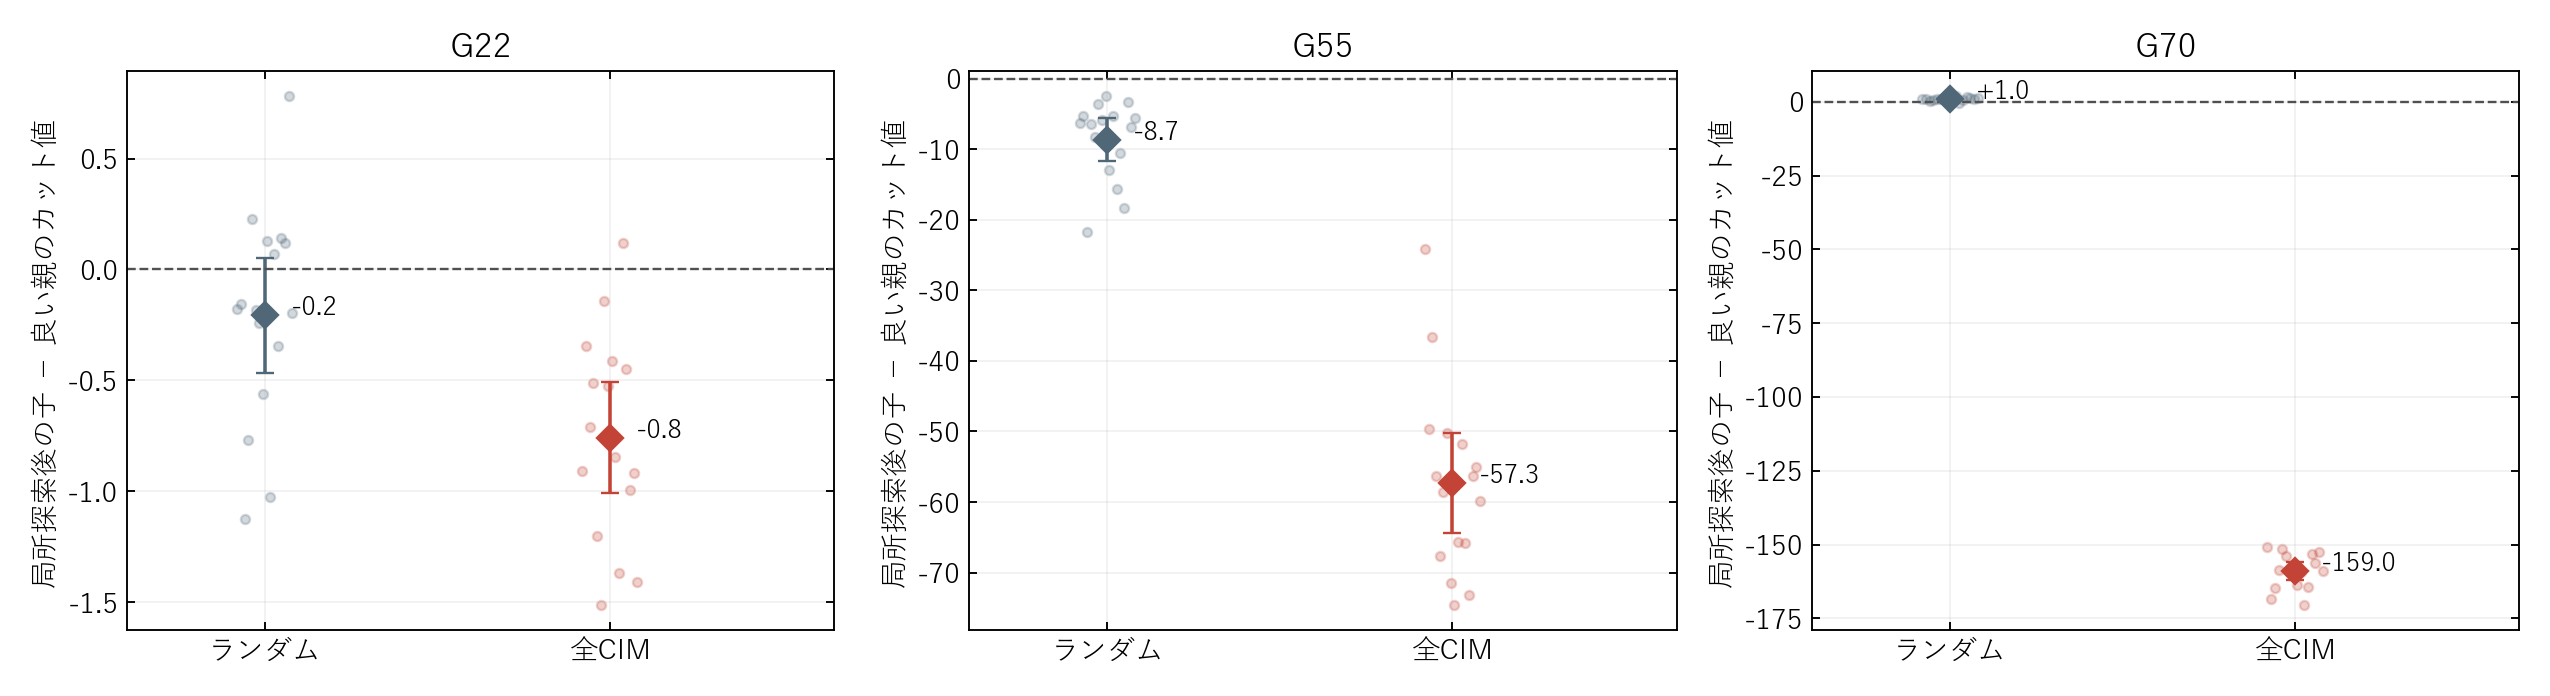
\includegraphics[width=\linewidth,height=80mm,keepaspectratio]{parent_differences.png}\par
\begin{center}\small
\begin{tabular}{llrrrr}\toprule
問題 & 初期集団 & 交叉後$-$良い親 & TS後$-$良い親 & TS後に良い親以上 & 悪化した子の回復\\\midrule
G22 & ランダム & -133.3 & -0.2 & 3461/4800 & 2674/4013\\
G22 & 全CIM & -104.3 & -0.8 & 3191/4800 & 2603/4212\\
G55 & ランダム & -495.9 & -8.7 & 1356/4800 & 1347/4791\\
G55 & 全CIM & -1268.8 & -57.3 & 152/4800 & 152/4800\\
G70 & ランダム & -279.8 & +1.0 & 3618/4800 & 3466/4648\\
G70 & 全CIM & -1546.6 & -159.0 & 0/4800 & 0/4800\\
\bottomrule\end{tabular}
\end{center}
{\footnotesize 「TS後に良い親以上」は該当件数/全子数。「悪化した子の回復」は、交叉で良い親より悪くなった子のうち、TS後に良い親以上に戻った件数/悪化した子数。薄い点はrunごとの300世代平均、ひし形は16run平均、誤差棒はrun単位の95\% $t$区間。初期品質はそろえておらず、多様性の因果効果を示す比較ではない。}

\clearpage
\heading{「改善した子」の意味を分けて、採用を確認する}{TSで子自身が良くなることと、親より良い子ができることは違う}
\textbf{TSで改善：}交叉直後の子より、局所探索後の子のカット値が高い。\\
\textbf{親を超えた：}局所探索後の子が、選択された両親の良い方よりも高い。\\
\textbf{採用：}集団更新処理DisQualが、集団の1個体を子に置き換えた。品質と最も近い他個体までの距離を併用して決める。

\begin{center}\small
\begin{tabular}{llrrrr}\toprule
問題 & 初期集団 & 全子の採用 & TS改善子の採用 & 親超え子の採用 & 過去最良更新子の採用\\\midrule
G22 & ランダム & 3848/4800 & 3060/4012（76.3\%） & 445/445（100.0\%） & 78/78（100.0\%）\\
G22 & 全CIM & 3520/4800 & 2932/4212（69.6\%） & 270/270（100.0\%） & 51/51（100.0\%）\\
G55 & ランダム & 3196/4800 & 3187/4791（66.5\%） & 1118/1122（99.6\%） & 397/397（100.0\%）\\
G55 & 全CIM & 1338/4800 & 1338/4800（27.9\%） & 136/139（97.8\%） & 40/40（100.0\%）\\
G70 & ランダム & 4493/4800 & 4341/4641（93.5\%） & 1302/1302（100.0\%） & 635/635（100.0\%）\\
G70 & 全CIM & 0/4800 & 0/4800（0.0\%） & 該当なし & 該当なし\\
\bottomrule\end{tabular}
\end{center}
{\small 採用欄は「採用件数/対象件数」。括弧はその対象内での採用率。「該当なし」は条件を満たす子が0個であり、採用率0\%とは異なる。過去最良の更新は、各runでそれまでに見つかった最良値を厳密に超えた件数。}

\textbf{G70・全CIMについて：}親を超えた子は一度も生まれていない。したがって、優れた子を採用処理が捨てたために停滞した、という結果ではない。交叉後に失った品質を、今回の局所探索では親の水準まで戻せていない。

{\small G70の300世代時点の平均最良カット値は、全CIM 9,495.19、ランダム 9,458.94。採用率の高低だけで、最終的な解の品質を判断しない。}

\textbf{この実験でまだ言えないこと：}CIMが出す解のどの構造がこの現象を生んだか、交叉や局所探索予算を変えると回復するかは未検証。今回の設定で起きている処理の流れを特定した結果である。

\begin{center}\small
\begin{tabular}{lrrrrr}\toprule
問題 & 集団サイズ & TS反復数 & 摂動待ち回数 & tenure係数 & 品質重み\\\midrule
G22 & 15 & 35,238 & 2159 & 40 & 0.8374\\
G55 & 6 & 58,453 & 930 & 13 & 0.4330\\
G70 & 8 & 41,152 & 521 & 11 & 0.6618\\
\bottomrule\end{tabular}
\end{center}

\vfill
{\footnotesize 1世代に各runで子を1個生成し、交叉→TS→採否を記録。集団の初期TSはこの4800件に含めない。同一run内の子は相関するため、件数4800を独立試行数とする有意差検定は行っていない。}

\clearpage
\heading{探索の途中で、回復と採用の傾向は変わるか}{4つの世代区間ごとに集計。上段はTS後の親との差、下段は全子の採用率}
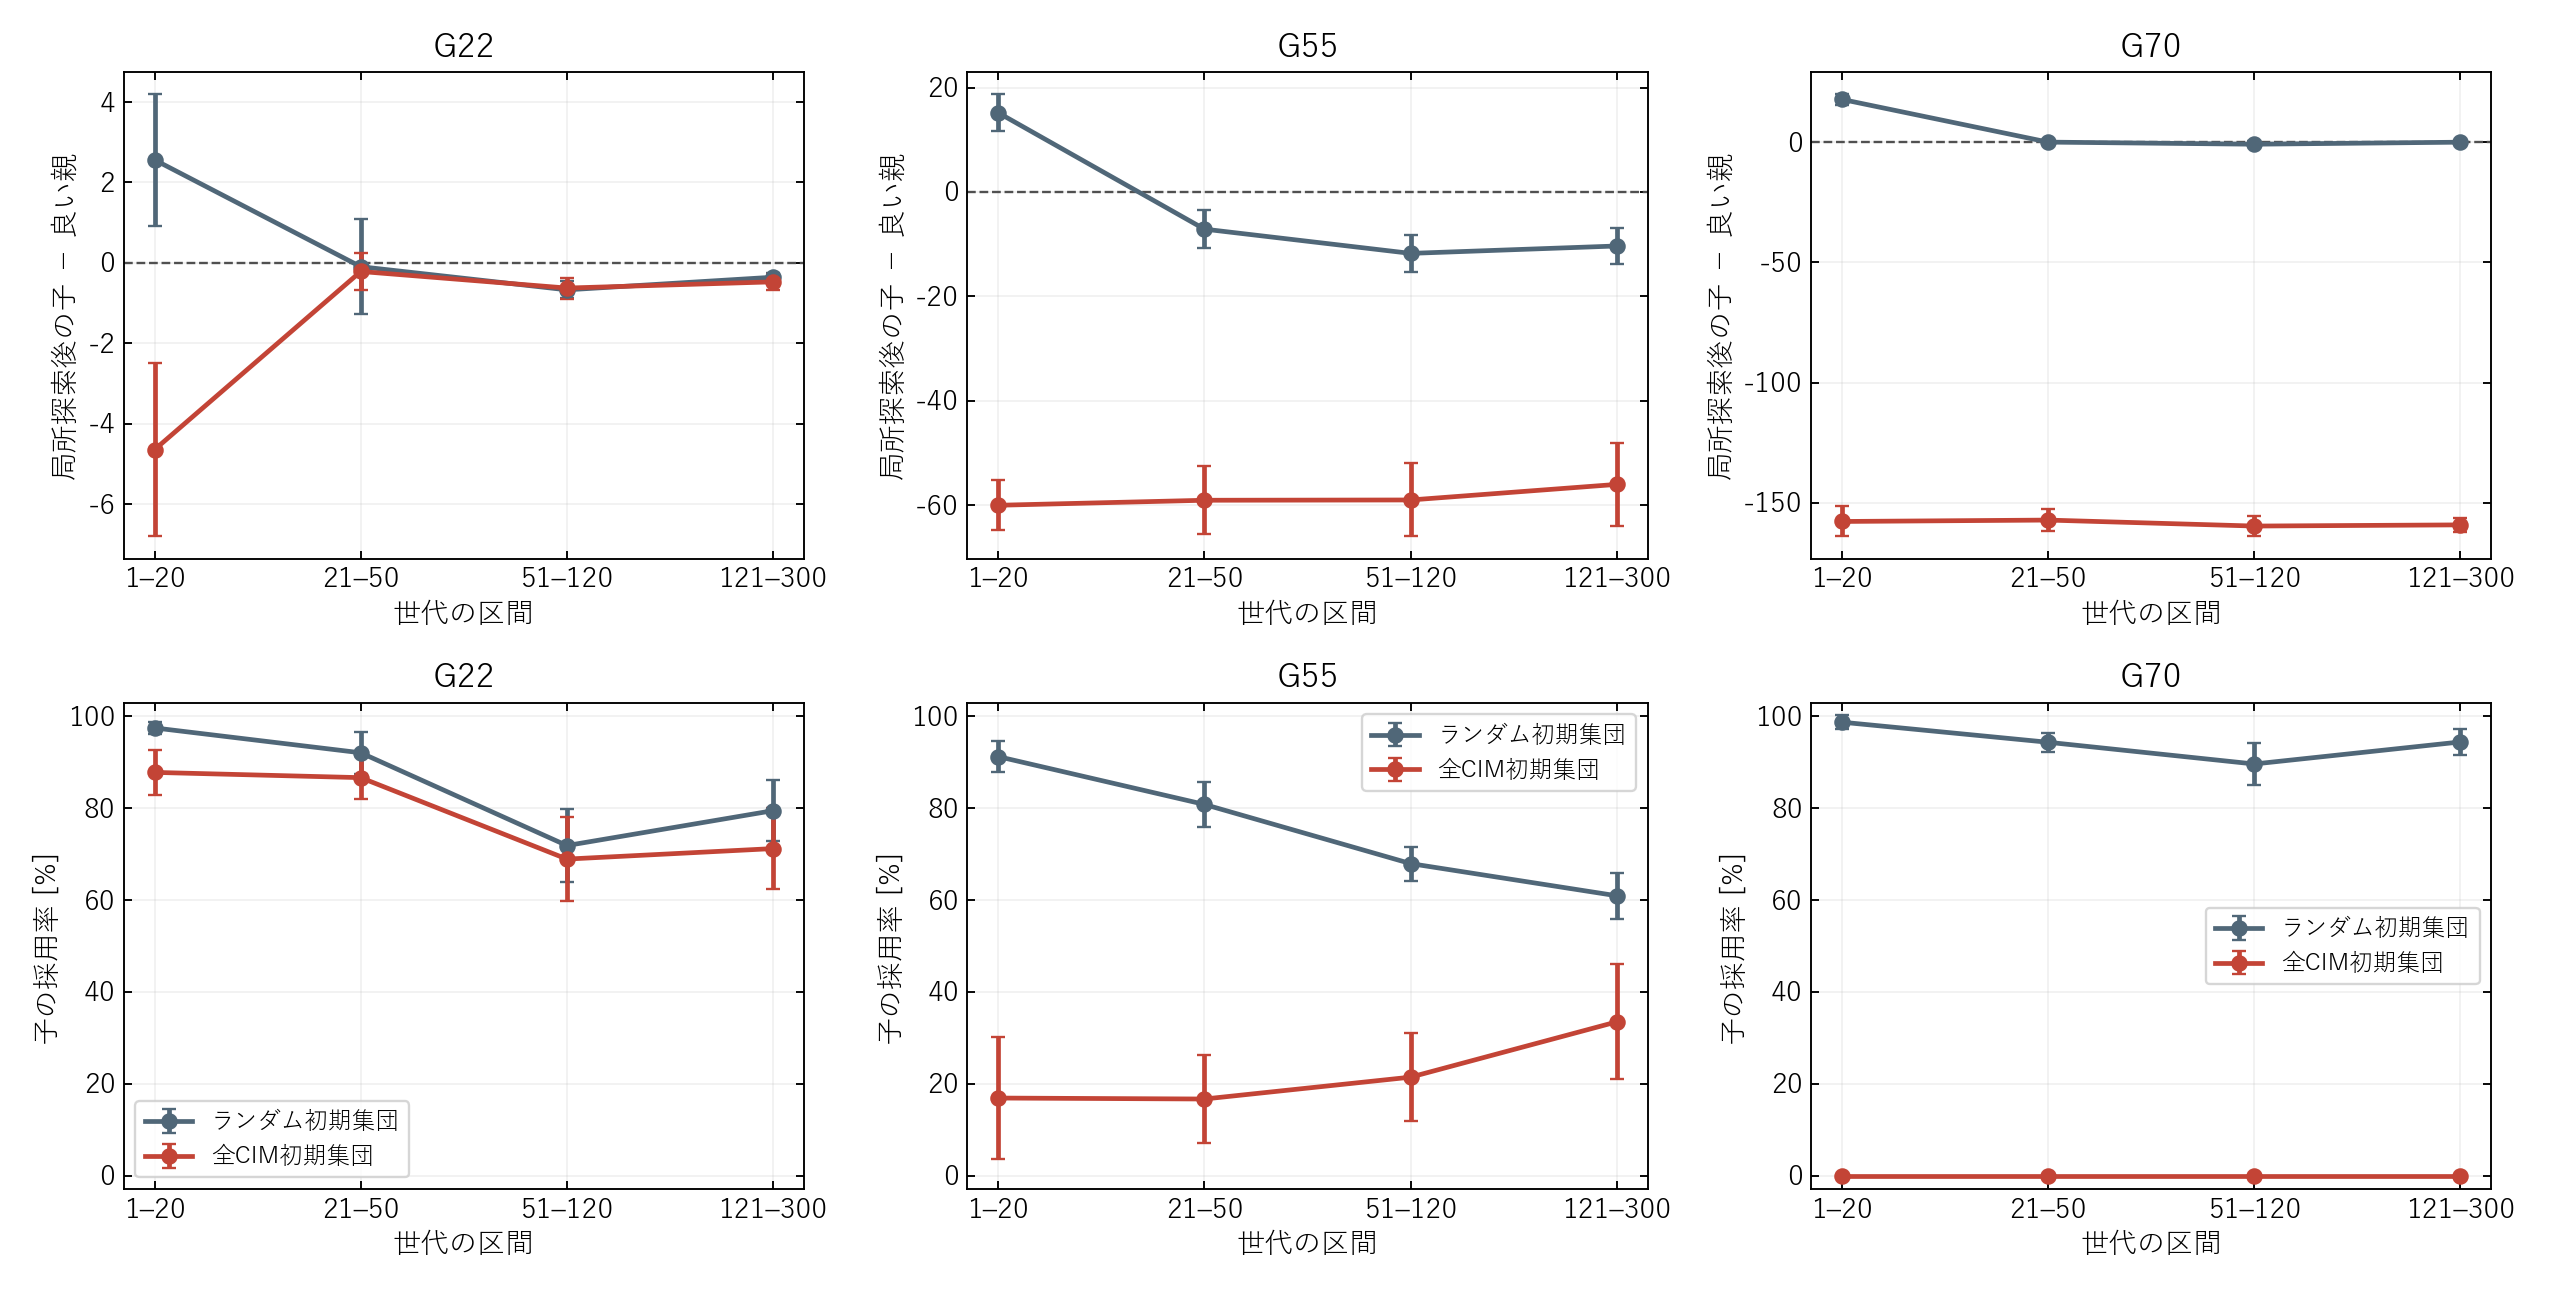
\includegraphics[width=\linewidth,height=123mm,keepaspectratio]{stage_trajectory.png}\par
{\footnotesize 点と誤差棒は、区間内をrunごとに平均してから求めた16run平均と95\% $t$区間。各条件の初期集団、CIM設定、GA設定、seedは前回と同じ。全世代の集団fitness・best履歴・保存した集団断面・最終解が前回と完全一致することを確認した。}

{\footnotesize 全子の両親・交叉直後・TS後のカット値を辺の和で独立に再計算し、報告値と照合。計測追加が結果を変えないこと等8件のテストに成功。全イベントの個体と数値、設定、ソースは本PDFと同じフォルダに保存。}
\end{document}
